\documentclass{article}%
\usepackage[T1]{fontenc}%
\usepackage[utf8]{inputenc}%
\usepackage{lmodern}%
\usepackage{textcomp}%
\usepackage{lastpage}%
\usepackage{graphicx}%
%
\title{ins (50)\_ Sidero{-}phore{-}mediated systems typically involve lo}%
\author{\textit{Yen Li Mei}}%
\date{10-31-1998}%
%
\begin{document}%
\normalsize%
\maketitle%
\section{There are two things that Australia and South Africa have in common}%
\label{sec:TherearetwothingsthatAustraliaandSouthAfricahaveincommon}%
There are two things that Australia and South Africa have in common. We have a lot of freedoms and we’re really the only country where you have to have separate silos to operate a business.\newline%
The other thing you have is that people from the outside just assume you don’t have a significant amount of work.\newline%
There’s a certain complacency and insecurity, people feel that you’re right, something you need to stay out of.\newline%
We have been working on these systems for over two years and at that time we had around 40 people on board.\newline%
Then a new thing came along and that was to plug into the existing systems and run multiple systems.\newline%
That led to the broader use of the standalone automated system, that we call HYE{-}CHO{-}PERO.\newline%
“HYE{-}CHO{-}PERO allows you to put together a system of your own, and it’s opened up an many, many systems for doing business in place.”\newline%
So what are you doing with this system?\newline%
I think our business is growing at quite a high rate… we’re expanding our business by bringing on people who have internet access and telecommuting.\newline%
We’re using our machines, or in some cases we are experimenting with thermostats.\newline%
How has this changed the way you organise your business?\newline%
I think it’s changed the way you organise your business. It allows you to divide, or integrate more and more of our business.\newline%
You say you’re a company, but how can you build such a complete machine to manage your organisation?\newline%
We are incredibly flexible, but we are very, very expensive. You need to be able to share services and you need to be able to manage everything with a firm payment plan.\newline%
My main difference with regards to that would be that we’re not going to sell everyone the full network of the consumer, if you want to have a fair pricing, you should be able to do that with lots of other people.\newline%
People that are familiar with your software don’t understand the problems they’re having, you should be able to change something and fix it or explain where it comes from.\newline%
So how do you think you can improve the existing systems?\newline%
People are having to behave in different ways, you can start without trying to add customers because there’s no self{-}management. You need to treat everyone the same way as a company and make sure we all have the same amount of space.\newline%
If you think we can get on an even keel, then we have to change everything. I think our industrial infrastructure in South Africa is important for addressing all three needs and there are hundreds of thousands of containers that can be converted to fast moving consumer goods.\newline%
When I first started my business I had 150 containers. Today it’s around 20 containers, so that’s twice as much.\newline%
We’re using a standard building, or the lower level of the building, to convert and we’re using some new capacity there.\newline%
Do you have any advice to other businesses looking to automate?\newline%
I think that aside from making people complacent, it’s about making people aware of your technology too.\newline%
A lot of companies, I don’t know if there are any, actually, that are going to automate {[}our processes{]} anymore.\newline%
But we’re doing it by doing it because we believe it’s much more efficient. I’m not saying we should try it because of it, I just don’t know.\newline%
That’s ok…in other businesses, where people are very concerned, where things are made difficult, that’s OK, I’ve tried before where I’ve seen the benefits.\newline%
If there are people that think we can only do 50, then we won’t be able to do more, but one of the things I love about Cyril Githouba as a leader is that you’re not different from anyone else, people are different, and there’s not as much fear on the consumer front.\newline%
That’s a pretty happy position for me.\newline%
As for the EPOWI system, in South Africa we only support the industry that we do on our computers.\newline%
Today we’re using Linux.\newline%
We’re not using Microsoft products, because Linux is now available, and we also use Java.\newline%

%


\begin{figure}[h!]%
\centering%
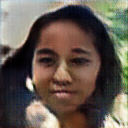
\includegraphics[width=120px]{./photos_from_epoch_8/samples_8_168.png}%
\caption{a man wearing a tie and a hat .}%
\end{figure}

%
\end{document}